\documentclass[Research_Module_ES.tex]{subfiles}
\begin{document}
\section{Simulations}
\label{Simulation1}
After the evaluation of the asymptotic properties of the different \textit{Cross-Validation} procedures we want to take a closer look to the finite sample performance. Therefore, we consider the following model:
\[
	y_i=\beta_1+x_{2i}\beta_2+x_{3i}\beta_3+x_{4i}\beta_4+x_{5i}\beta_5+\varepsilon_i
\]
where $i=1,\ldots,n$ with $n$ being the total number of observations. The error terms $\varepsilon_i$ are iid form $N(0,1)$,  $x_{ki}$ is the i'th value of the k'th regression variable and all $x_{ki}$, $k=1,\ldots5$, are generated from different normal distributions\footnote{See Appendix II}. Moreover, we assume that
\[
	\beta=(\beta_1,\beta_2,0,0,0)^\prime
\]
where $\beta_1,\beta_2$ are unequal to zero. So the Model with the best predictive ability have to be chosen out of five possible repressors $\{x_1,\ldots,x_5\}$. \\
\\
For the different simulations we consider the five model section methods: CV(1), MCCV($n_\nu$),BICV($n_\nu$) and since they are popular in praxis AIC,BIC as benchmark. Also note that $n_v=n-\lfloor n^{3/4}\rfloor$.

\subsection{Ability of distinguishing between Category I and II }
In the first simulation we want to take a closer look at the probability given in Theorem (\ref{THM_Consistency of $CV(1)$} ) III. We saw that for $n\to\infty$ the different \textit{Cross-Validation} methods are perfectly able to distinguish between Category I and II, hence the probability of choosing a model from Category I equals zero. But how good will \textit{Cross-Validation} perform with only finite information and will all methods behave similar?\\
\\
Figure \ref{Simulation1} shows how the probability of choosing a Category II model behaves for different sample sizes. To calculate these probabilities we repeat the procedure of model selection 2000 times for each sample size and plot the relative frequencies.\footnote{Note that for each of the 200 iterations a completely new sample was generated.}

As we can see in Figure \ref{Simulation1}, the probabilities of choosing a Category II model is converging to 1 for all five methods. Moreover all methods perform quite similar in distinguishing between the two models, only the MCCV seems to be slightly worse then the other ones. The purpose of this is the smaller trainings set of MCCV which is chosen with $\lfloor n^{3/4}\rfloor$. Therefore MCCV only predicts $\Gamma_{\alpha,n-n_v}$, which is a less accurate estimate than $\Gamma_{\alpha,n}$ which is calculated by the other methods. 
\begin{figure}[h]
	\label{Simulation1}
	\centering
	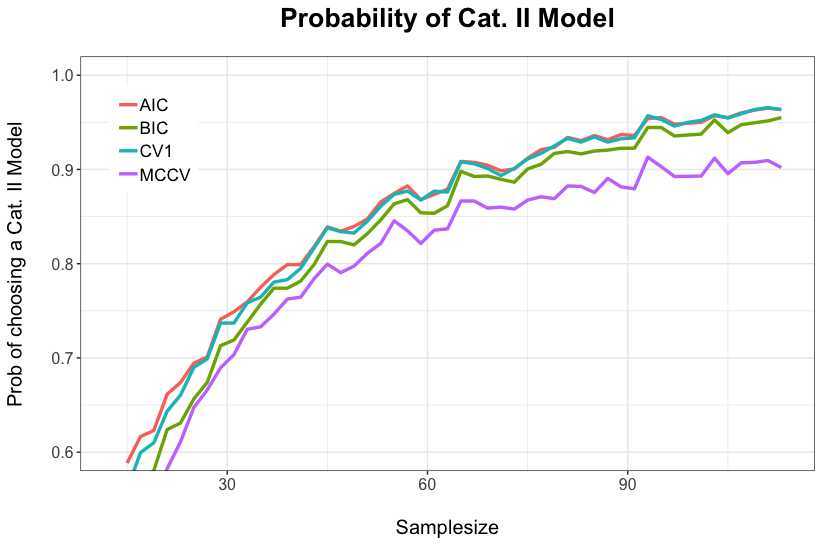
\includegraphics[width=1\textwidth]{Simulation1.png}\\
\caption{Probability of Choosing Cat II Models}
\end{figure}
\subsection{Ability of distinguishing  between Category II Models}
In chapter \ref{Simulation1} we showed that all five methods of model section are quite good in distinguishing between models form Category I and II, hence they all picked Category II models with large probabilities. \\
\\
For the next simulation we only consider models in Category II\footnote{To be more precisely: We only allow Category II models as choice for the model selection problem.}. To rectify this assumption we choose a large sample size of $n=500$, hence we already mentioned that for such large sample size the probability of choosing a Category II model is close to one.\\
\\
Figure \ref{Simulation2} shows the probabilities of choosing models of a certain dimensionality for all five methods\footnote{Therefore we repeated the model selection 2000 times for different samples and counted how often models with certain dimensionality were chosen.}. Since we only look at models from Category II we know that the model with the smallest dimensionality has to be  the true model $M_\ast$. In this sense we denote a model with a dimensionality higher by one then the true models dimensionality with $M_\ast+1$.\\
As we can see, both AIC and CV(1) perform almost equivalent\footnote{These similar performance is not unexpected since \cite{stone1977asymptotic} showed that AIC and CV(1) are asymptotically equivalent} and tend to pick to large models. BIC and MCCV  perform better, both pick the true model with a probability close to one and they choose to large models in only few cases. Within our 2000 simulations there was not a single case where BIC and MCCV chooses models with a dimensionality larger then $M_\ast+1$.
\begin{figure}[h]
	\label{Simulation2}
	\centering
	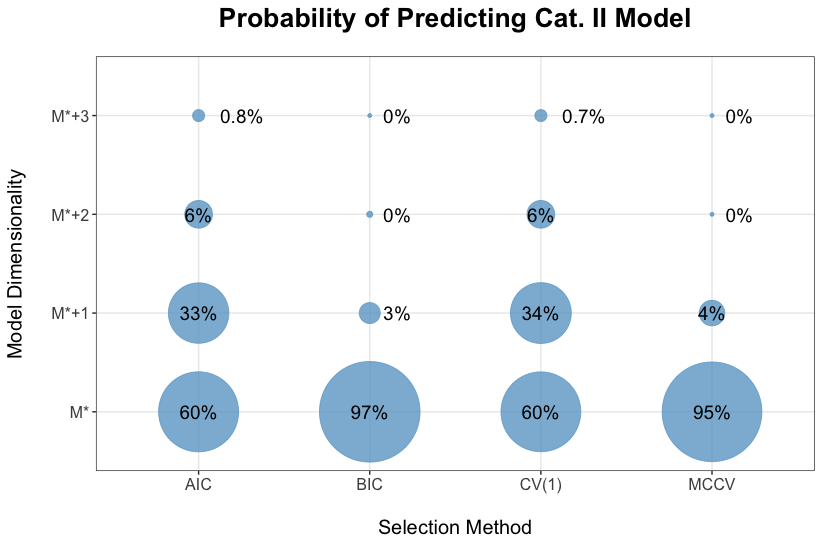
\includegraphics[width=1\textwidth]{Simulation2.png}\\
	\caption{Probability of Choosing diffrent Models form Cat II}
\end{figure}
\subsection{R Code Efficiency}
Beside asymptotic analyses, the performance of the small sample properties is an important aspect of statistical research. An often used approach to analyse such small sample properties are simulation studies, like we did in the previous chapters.\\
\\
Due to inefficiencies of our R code we had to spend weeks of computing time. Therefore one import part of our work was to find ways in order to speed up our R code and reduce it's computational complexity.\\
\\
The statistical software R is popular in statistics, although it's slow in comparison to other languages. The reason for the popularity of R is its high flexibility and simplicity.

To speed R up, our first approach was to look at the basic commands we used and to make them less flexible. To do so we used the command {\itshape package :: function}. This command shows the code behind predefined R commands, for example the {\itshape sample()} command \footnote{{\itshape sample(x,size)} draws randomly {\itshape size} elements from the set {\itshape x} } we get:
\begin{lstlisting}
> base::sample
function (x, size, replace = FALSE, prob = NULL) 
{
	if (length(x) == 1L && is.numeric(x) && is.finite(x) && x >= 
		1) {
		if (missing(size)) 
			size <- x
		sample.int(x, size, replace, prob)
	}
	else {
		if (missing(size)) 
			size <- length(x)
		x[sample.int(length(x), size, replace, prob)]	
	}
}
\end{lstlisting}
We see that {\itshape sample} checks additional conditions beside it's main purpose, since we do not need this, we can simplify it by using {\itshape x[sample.int(length(x), size)}.\\
\\
One other example is the matrix vector multiplication. R for example would compute $P=X(X^\prime X)^{-1}X^\prime y$ by first solving $X(X^\prime X)^{-1}$, then multiplying the outcome with $X^\prime$ and finally multiplying with $y$. This is inefficient due to the dimensionality of the out coming intermediate results, a more efficient way of computing is $P=X[ (X^\prime X)^{-1}(X^\prime y)]$.
\\
\\
The most time consuming aspect of our simulations is the process of models selection. Its natural to start there with the search of inefficiencies










\newpage



%BEISPIELTABELLE habe mal ein paar willkürliche sachen in der ersten zeile eingegeben, die wir später einfach nur ersetzen müssen, die letzten zeilen hab ich jetzt nicht weiter mit beispielzahlen gefüllt (ist noch eine alte tabelle von mir)
\begin{table}[htb]
	\begin{tabular}{lcccccc}
		\toprule
		\midrule
		\textbf{\scriptsize Initial $\beta$}
		&\textbf{\scriptsize Model $\mathcal{M}_\alpha$}&\textbf{\scriptsize Category}
		&\textbf{\scriptsize CV(1)}
		&\textbf{\scriptsize MCCV($n_\nu$)}
		&\textbf{\scriptsize APCV($n_\nu$)}
		&\textbf{\scriptsize BICV($n_\nu$)}\\
		$~$ &\textbf{\scriptsize $\alpha=\{...\}$} 
		\\\midrule\midrule
		
		{\scriptsize $\beta=(1,2,3,4,5,6)^\prime$}& \scriptsize alpha-werte & \scriptsize eins-oder-zwei &\scriptsize WertSpalte1 & \scriptsize WertSpalte2 &\scriptsize WertSpalte3 & \scriptsize WertSpalte4\\
		
		~& \scriptsize alpha-werte & \scriptsize eins-oder-zwei &\scriptsize WertSpalte1 & \scriptsize WertSpalte2 &\scriptsize WertSpalte3 & \scriptsize WertSpalte4\\
		
		~& \scriptsize alpha-werte &\scriptsize eins-oder-zwei & \scriptsize WertSpalte1 &\scriptsize WertSpalte2 & \scriptsize WertSpalte3 &\scriptsize WertSpalte4\\
		& & & & & &\\
		
		%ALTE tabelle
		{\scriptsize Initialset $\{X_{1},X_{2},X_{3},X_{4}\}$}\\
		{\scriptsize I-Score vor der Verwerfung}& \scriptsize 3,6896 & \scriptsize 7,1186 &\scriptsize 13,1224 & \scriptsize 14,2844 & & \\
		\scriptsize Verworfene Variable& \scriptsize $X_{3}$ &\scriptsize $X_{1}$ & \scriptsize $X_{2}$ &\scriptsize $X_{4}$ & & \\
		& & & & & &\\
		{\scriptsize Initialset $\{X_{1},X_{2},X_{3},X_{6}\}$}\\
		{\scriptsize I-Score vor der Verwerfung}& \scriptsize 2,0536 & \scriptsize 2,7195 &\scriptsize 3,9136 & \scriptsize 6,9534 & & \\
		\scriptsize Verworfene Variable& \scriptsize $X_{3}$ &\scriptsize $X_{6}$ & \scriptsize $X_{1}$ &\scriptsize $X_{2}$ & & \\
		& & & & & &\\
		{\scriptsize Initialset $\{X_{1},X_{3},X_{6}\}$}\\
		{\scriptsize I-Score vor der Verwerfung}& \scriptsize 0,8767 & \scriptsize 0,8681 &\scriptsize 0,1324 & & & \\
		\scriptsize Verworfene Variable& \scriptsize $X_{1}$ &\scriptsize $X_{6}$ & \scriptsize $X_{3}$ & & & \\
		\bottomrule
	\end{tabular}
	\caption{Verwerfungsprozess für vier Fälle}
\end{table}

\subsection{Different $n_{\nu}$}


\subsection{Consistency}

\subsection{Category \RM{1} - Simulation}


\end{document}